% !TEX root = DesignDocument.tex

\chapter{Overview and concept of operations}
The UAV Lander project requires the autonomous take-off, waypoint navigation, and landing of a UAV. Most of this can be provided by built-in capabilities of a flight controller. However, the larger problem within this project is to land the UAV within $\pm$.1m of the center of the landing pad and with minimal error in orientation. This section will provide the reader with a broad overview of the technologies relating to the objectives of this project.


\section{Scope}
This document provides the reader with an understanding of the UAV Landing Project to include the purpose of the project, the project's main system components, how these components will function together, and a description of the technologies used to develop this project. This document is limited to the technologies that are/will be implemented on the build of the UAV. Necessarily, this document does not extend to some of the development tools or include details concerning the technologies involved with the landing pad.  

\section{Purpose}
The purpose of this project is to develop software that will enable a UAV to autonomously take-off, navigate through some number of user defined waypoints, return to the landing pad, and land with $\pm .1$m of the center of the landing pad with $\pm 15^{\circ}$ of the correct orientation. The platform for testing this software will be a carbon fiber frame hexrotor controlled by a flight controller augmented with input from an ODroid.  

\subsection{Flight Controller}
The flight controller unit(FCU) will control the manual or autonomous flight of the UAV. The autonomy, specifically, will address the functions of take-off and waypoint navigation. Autonomous landing using relatively inexpensive flight controllers can typically only provide an accuracy of $\pm$10m, though many users claim that accuracy is half of that. \\

\noindent The team has selected the Pixhawk flight controller, with a GPS peripheral. The GPS unit will allow for waypoint navigation controlled by a ground control station(which is a piece of software to tell the UAV where to go and what to do). The Pixhawk includes:
\begin{itemize}
\item Pixhawk autopilot
\item Buzzer
\item Safety switch button
\item 3DR power module with XT60 connectors and 6-position connector cable
\item Extra 6-position cable to connect a 3DR GPS+Compass module
\item Micro USB cable
\item SD card and adapter
\item Mounting foam
\item 3-wire servo cable
\item I2C splitter module with cable
\end{itemize}
It also includes the features:
\begin{itemize}
\item Advanced 32 bit ARM Cortex® M4 Processor running NuttX RTOS
\item 14 PWM/servo outputs (8 with failsafe and manual override, 6 auxiliary, high-power compatible)
\item Abundant connectivity options for additional peripherals (UART, I2C, CAN)
\item Integrated backup system for in-flight recovery and manual override with dedicated processor and stand-alone power supply
\item Backup system integrates mixing, providing consistent autopilot and manual override mixing modes
\item Redundant power supply inputs and automatic failover
\item External safety button for easy motor activation
\item Multicolor LED indicator
\item High-power, multi-tone piezo audio indicator
\item microSD card for long-time high-rate logging
\end{itemize}

\noindent The large reason behind using the Pixhawk is that there is an established API(Mavlink) to send commands and receive commands with the flight controller. Mavros will provide a convenient handle so we can take advantage of the built-in autonomy for take-off and waypoint navigation, yet still have the ability to interrupt the built-in autonomy when reaching the landing zone. 

\subsection{ODroid}
The ODroid XU4 is small board computer featuring:
\begin{itemize}
\item Samsung Exynos5422 Cortex™-A15 2Ghz and Cortex™-A7 Octa core CPUs
\item Mali-T628 MP6(OpenGL ES 3.0/2.0/1.1 and OpenCL 1.1 Full profile)
\item 2Gbyte LPDDR3 RAM PoP stacked
\item eMMC5.0 HS400 Flash Storage
\item 2 x USB 3.0 Host, 1 x USB 2.0 Host
\item Gigabit Ethernet port
\item HDMI 1.4a for display
\end{itemize}
\noindent This computer, with 8 cores, is enough to run a full Ubuntu 14.04 install, which is needed to run a ROS Indigo/Jade Distro. This computer will also be connected to one or two cameras, and be responsible for processing the image stream, calculating needed landing instructions, and passing those instructions to the Flight Controller.

\subsection{Hexrotor}
The hexrotor is the platform our team will using to test and demonstrate our autonomous landing implementation(take-off and waypoint will be handled by the flight controller's built-in autonomy). The hexrotor was decided upon as being more stable, and therefore more desirable, than a quadrotor design. The hexrotor specifically includes:
\begin{itemize}
\item Turnigy Talon Hexcopter (V1.0) Carbon Fiber Frame(625mm diameter)
\item 6 AeroSky Performance Brushless Multi-Rotor Motor MC3525 850KV
\item 6 Exceed RC Proton 30A Brushless ESC Speed Controller
\item Hexacopter Power Distribution Board
\item APM Power Module with XT60 Connectors Kit
\item 3 Each Carbon Fiber Propeller 10x4.7 Black (CW/CCW)
\item Battery
\end{itemize}
A custom cage will be designed and constructed to house the Pixhawk, GPS, and ODroid XU4. 

\subsection{Robot Operating System(ROS)}
The Robot Operating System is a pseudo-operating system that provides libraries and tools allowing a fast integration of hardware. ROS creates a network to allow the passing of information between nodes that either push or pull information as needed. Our implementation will use ROS to create a network of nodes that will push or pull information, such as pulling images to calculate direction and distance needed to reach the landing pad. A node will be responsible for pushing that information to the flight controller via MavROS.

\subsection{Mavlink}
Mavlink(Micro Air Vehicle link) is a message protocol for communicating with small unmanned vehicles including ground vehicles, planes, and helicopters. Mavlink is often used for many flight controllers, providing a good interface for sending commands, as well as receiving information from the flight controller. The team will be using MavROS in implementation, which is Mavlink, but with a ROS wrapper. This will allow us to keep our ODroid side implementation in a ROS environment.

\section{Systems Goals}
The goals of this project:
\begin{enumerate}
\item Autonomously take-off from landing pad.
\item Autonomously navigate through a series of waypoints.
\item Autonomously return to the landing pad.
\item Autonomously land within $\pm$.1m of the center of the pad.
\item Autonomoulsy land with the correct orientation $\pm 15^{\circ}$.
\end{enumerate}

\section{System Overview and Diagram}
The flight controller will be responsible for take-off and waypoint navigation. As described earlier, the Pixhawk flight controller is capable of receiving instructions through the use of a GUI, a ground control station, to establish take-off, waypoint navigation, including navigation back to the landing pad. The ODroid will be receiving and listening to the instructions(or missions) being executed by the flight controller. Reaching the last waypoint(the landing pad), the ODroid will interrupt the autonomous landing on the flight controller. The ODroid will use a camera and the stream of images to estimate movements to reach the landing pad, on center and with correct orientation. These instructions will be sent to the flight controller. The instructions will continuously be sent to the flight controller until the UAV has landed(Fig.~\ref{overviewdiag}).\\ 

\begin{figure}[h]
\begin{center}
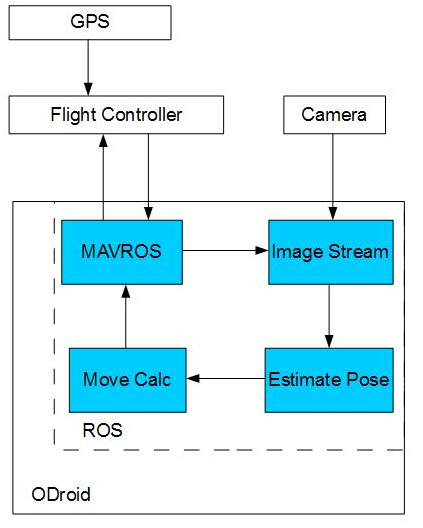
\includegraphics[width=0.5\textwidth]{broad_approach1.PNG}
\end{center}
\caption{Communication between Flight Controller and ODroid \label{overviewdiag}}
\end{figure}

\section{Technologies Overview}
\textbf{HARDWARE DEPENDENCIES:}
\begin{itemize}
\item 3DR Pixhawk Flight Controller - The flight controller will provide the ability to fly the hexrotor craft manually and autonomously. \href{https://store.3drobotics.com/products/3dr-pixhawk}{More information here}.
\item 3DR GPS - Provides global coordinates, which is essential for gps defined waypoint navigation. \href{https://store.3drobotics.com/products/3dr-gps-ublox-with-compass}{More information here}.
\item ODroid XU4 - This will serve as the host for the ROS framework for processing image information, calculating move instructions, and sending those instructions to the flight controller. \href{http://www.hardkernel.com/main/products/prdt_info.php}{More information here}.
\item Camera - Currently a camera has not been selected. The camera will need the capability of clearly recognizing lights and discriminating color at a distance of up to 10m at at least 30fps. 
\end{itemize}

\noindent\textbf{SOFTWARE DEPENDENCIES:}
\begin{itemize}
\item Ubuntu 14.04 - ROS necessitates the use of this OS. This will be the environment found on the ODroid. \href{https://wiki.ubuntu.com/TrustyTahr/ReleaseNotes}{More information here}.
\item OpenCV - This open source library provides built-in image processing that will allow the team to process images from the camera to compute move instructions.  \href{http://opencv.org/}{More information here}.
\item Robot Operating System(ROS) - ROS will serve as the structure for the program so that we can construct a framework to process an image, derive some decision from the image, and send the instruction to the flight controller. \href{http://www.ros.org/}{More information here}.
\item Mavlink - A protocol to communicate with the flight controller, such as to send instructions or receive some information about the flight. \href{https://pixhawk.ethz.ch/mavlink/}{More information here}.
\end{itemize}

